\setcounter{framenumber}{163}
\begin{frame}
	\maketitle
\end{frame}

\begin{frame}{Overview}
\tableofcontents
\end{frame}

\section{Rehash}
\begin{frame}{Rehash}
	
 \begin{itemize}

	\item Models in propositional logic are \emph{valuations}: functions from sentence letters to truth-values.
	
	\item We can calculate the value of a formula under a valuation recursively using the Boolean \emph{truth-functions}.
	
	\item The validity of inferences over formal languages can be understood in terms of the concept of logical consequence.
	
	\item \alert{A set of formulas entails a formula iff in every valuation s.t. all the members of the set have value 1, the formula has value 1.}
	
	\item \alert{A formula is a logical truth if it's a consequence of $\emptyset$.}
	
	\item The question whether a given set of premises entails a conclusion can be reduced to the question whether the conditional with the conjunction of the premises as the if-part and the conclusion as the then-part is logically valid.
		
	\item The method of truth-tables allows us to decide in finitely many steps whether a given formula is valid. This gives us a decision procedure for propositional logic.
	
	
\end{itemize}

\end{frame}
		

\section{6 Tableaux for Propositional Logic}
\subsection{6.1 Proof Systems}

\begin{frame}{6.1 Proof Systems}

	\begin{itemize}
	
		\item (6.1.1) The aim is formulate \emph{inference rules} that allow us to derive the conclusion from the premises in all (and only) the valid inferences.

		\item Proof theory provides a \emph{syntactic} approach to validity.
				
		\item This is good for implementability:
		
		\begin{center}
			\begin{tabular}{c c c}
				
				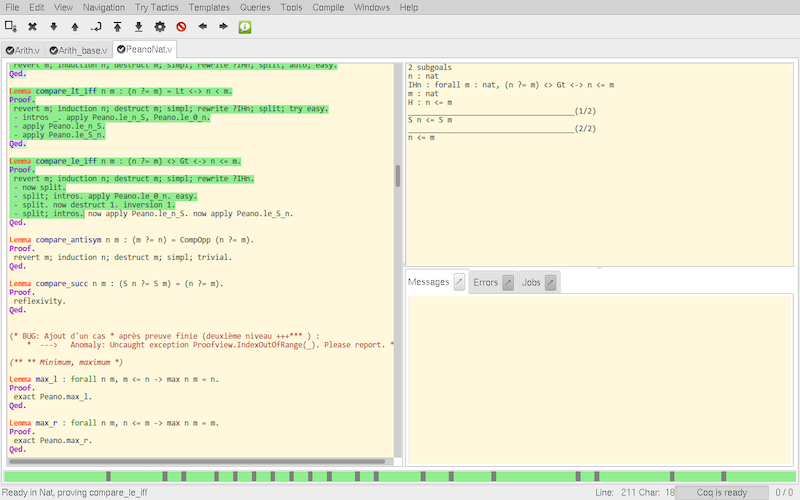
\includegraphics[height=15ex]{coq-screenshot} & &					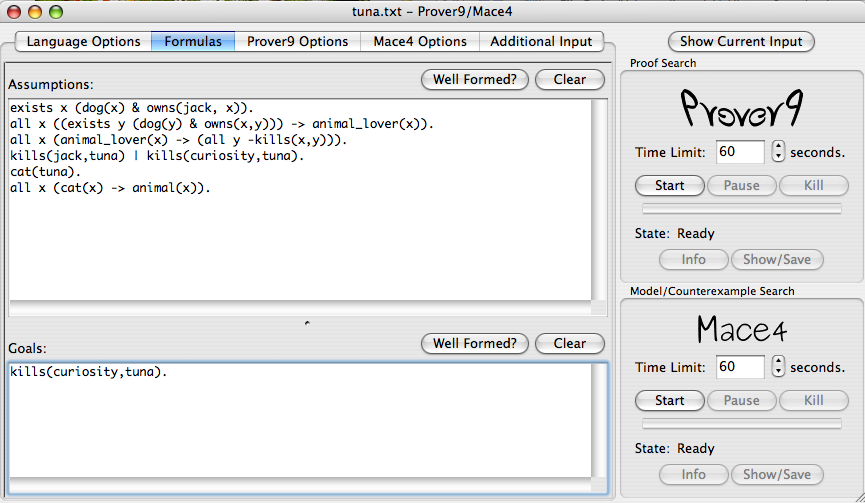
\includegraphics[height=15ex]{prover9-mace4-screenshot} \\
				{\tiny \textcopyright~Wiki author \texttt{Matj\v{e}j Grabovsk\'y}, LGPLv2.1} & &{\tiny \textcopyright~\url{https://slidewiki.org/user/OlliG}, CC BY-SA 4.0} \\[1ex]

				Proof Assistants (Coq) &\qquad & Theorem Provers (Prover9)

			\end{tabular}
		\end{center}
		
		\item There are also several mathematical upshots (e.h. consistency of arithmetic).
						
		\end{itemize}

\end{frame}

\begin{frame}{Hilbert Systems}

	\begin{itemize}
	
		\item (6.1.2) Modeled after axiomatic reasoning: axioms + inference rules.
	
		\item Hilbert calculus for propositional logic:
		
		 \begin{description}

						\item[Hilbert$_1$] $\phi\to (\psi\to \phi)$

						\item[Hilbert$_2$] $(\phi\to (\psi\to \chi))\to((\phi\to \psi)\to (\phi\to \chi))$

						\item[Hilbert$_3$] $(\neg \phi\to \neg \psi)\to (\psi\to\phi)$				
						
						\item[Modus Ponens.] From $\phi$ and $(\phi\to\psi)$ infer $\psi$.
						
						\item[Definitions.] From $(\phi\land\psi)$ infer $\neg(\phi\to\neg\psi)$ and vice versa; from $(\phi\lor\psi)$ infer  $(\neg\phi\to\psi)$ and vice versa; and from $(\phi\leftrightarrow\psi)$ infer $((\phi\to\psi)\land(\psi\to\phi))$ and vice versa.

		\end{description}
		
		\item A \emph{proof} in the Hilbert system is a sequence of formulas such that each formulas is either an axiom (in our case, an instance of \textbf{Hilbert}$_\text{1--3}$) or inferred from some formulas earlier in the proof via an inference rule (in our case, \textbf{Modus Ponens}  or \textbf{Definitions}). Notation: $\vdash_H\phi$
	
	\end{itemize}

\end{frame}

\begin{frame}{Example}

\begin{center}
		\begin{tabular}{c}
		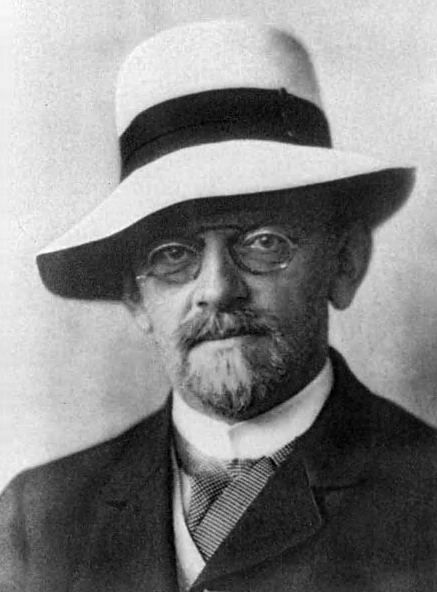
\includegraphics[width=10ex]{hilbert}\\[-1ex]
		{\tiny $\not\hspace{-1ex}\textcopyright$ David Hilbert, work in public domain}
		\end{tabular}
		\vspace{2ex}
		
		$\vdash_H p\to p$
		\end{center}
		
		
			\begin{enumerate}[1.] 

	\item $((p \to ((p \to p) \to p)) \to ((p \to (p \to p)) \to (p \to p)))$ 

	\item[] \ \hfill (Axiom 2. with $\phi=p, \psi=(p\to p),$ and $\chi=p$)

	\item $(p \to ((p \to p) \to p))$ \hfill (Axiom 1. with $\phi=p$ and $\psi=(p\to p)$)

	\item $((p \to (p \to p)) \to (p \to p))$ \hfill (From 1. and 2. by MP.)

	\item $(p \to (p \to p))$ \hfill (Axiom 1. with $\phi=p$ and $\psi=p$.)

	\item $(p \to p)$\hfill (From 3. and 4. by MP.)

\end{enumerate}

\end{frame}

\begin{frame}{Sequent Calculus}

	\begin{itemize}
	
		\item (6.1.4) Reasoning \emph{about} consequence using sequents $\Gamma\Rightarrow\Delta$.
		
		\item  $\phi_1,\mathellipsis,\phi_n\Rightarrow\psi_1,\mathellipsis, \psi_m$ means $\phi_1\land\mathellipsis\land\phi_n\vDash\psi_1\lor\mathellipsis\lor\psi_m$
	
		\item Calculus for propositional logic: $\phi\Rightarrow\phi$ +
		
		{\tiny\begin{center}
		\begin{tabular}{c c c}
			\infer[Weak L]{\Gamma\cup\{\phi\}\Rightarrow \Delta}{\Gamma\Rightarrow\Delta} & \infer[Weak R]{\Gamma\Rightarrow \Delta\cup\{\phi\}}{\Gamma\Rightarrow\Delta}\\[2ex]
			
			\infer[Cut]{\Gamma\cup\Gamma'\Rightarrow\Delta,\Delta'}{\Gamma\Rightarrow \{\phi\}\cup \Delta & \{\phi\}\cup\Gamma'\Rightarrow\Delta'}\\[2ex]
		
			
				\infer[\neg L]{\Gamma\cup\{\neg\phi\}\Rightarrow\Delta}{\Gamma\Rightarrow\Delta\cup\{\phi\}} & \infer[\neg R]{\Gamma\Rightarrow\Delta\cup\{\neg\phi\}}{\Gamma\cup\{\phi\}\Rightarrow\Delta} \\[2ex]
			
				\infer[\land L]{\Gamma\cup\{\phi\land \psi\}\Rightarrow \Delta}{\Gamma\cup\{\phi,\psi\}\Rightarrow \Delta} & \infer[\land R]{\Gamma\cup\Gamma'\Rightarrow \{\phi\land \psi\}\cup\Delta\cup\Delta'}{\Gamma\Rightarrow \{\phi\}\cup\Delta & \Gamma'\Rightarrow \{\psi\}\cup\Delta'}\\[2ex]
				
				 \infer[\lor L]{\Gamma\cup\Gamma'\cup \{\phi\lor \psi\}\Rightarrow\Delta\cup\Delta'}{\Gamma\cup \{\phi\}\Rightarrow\Delta & \Gamma'\cup\{\psi\}\Rightarrow \Delta'} & \infer[\lor R]{\Gamma\Rightarrow \Delta\cup\{\phi\lor \psi\}}{\Gamma\Rightarrow \Delta\cup\{\phi,\psi\}}\\[2ex]
				 
				 \infer[\to L]{\Gamma\cup\Gamma'\cup\{\phi\to\psi\}\Rightarrow\Delta\cup\Delta'}{\Gamma\Rightarrow \{\phi\}\cup\Delta' & \Gamma'\cup\{\psi\}\Rightarrow \Delta'} & \infer[\to R]{\Gamma\Rightarrow \{\phi\to\psi\}\cup\Delta}{\Gamma\cup\{\phi\}\Rightarrow\{\psi\}\cup\Delta}
				
			\end{tabular}
			\end{center}
	}
	
	\item A proof is a tree whose leafs are axioms and that's constructed according to the rules. $\Gamma\vdash_G\Delta$ means there's a proof that ends in $\Gamma\Rightarrow\Delta$.
	\end{itemize}


\end{frame}

\begin{frame}{Example}

\begin{center}
		\begin{tabular}{c}
		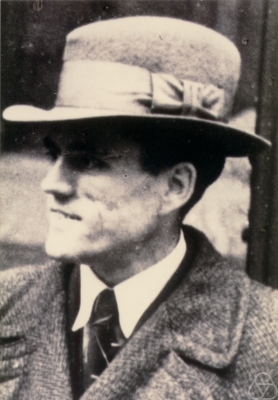
\includegraphics[width=10ex]{gentzen}\\[-1ex]
		{\tiny $\textcopyright$ Eckart Menzler-Trott, Gerhard Gentzen, \texttt{CC BY-SA 2.0 DE}}
		\end{tabular}
		\vspace{2ex}
		
		$\neg(p\lor q)\vdash_G \neg p\land \neg q$
		\end{center}
		
		
\begin{center}
		\begin{tabular}{c}
		\infer[\land R]{\neg(p\lor q)\Rightarrow \neg p\land \neg q}{\infer[\neg R]{\neg(p\lor q)\Rightarrow \neg p}{\infer[\neg L]{\neg (p\lor q),p\Rightarrow \emptyset}{\infer[\lor R]{p\Rightarrow p\lor q}{\infer[Weak R]{p\Rightarrow p,q}{p\Rightarrow p}}}} & \infer[\neg R]{\neg(p\lor q)\Rightarrow \neg q}{\infer[\neg L]{\neg (p\lor q),q\Rightarrow \emptyset}{\infer[\lor R]{q\Rightarrow p\lor q}{\infer[Weak R]{q\Rightarrow p,q}{q\Rightarrow q}}}}}
		\end{tabular}
	\end{center}
\end{frame}

\begin{frame}{Natural Deduction}

	\begin{itemize}
	
		\item (6.1.6) Modeled after natural reasoning using assumptions. Only rules.
		
		\item System for propositional logic:
		
				\begin{center}
{\tiny
			\begin{tabular}{c c c}
				
				\infer[EFQ]{\psi}{\phi & \neg \phi} & & \infer[Biv]{\psi}{\infer*{\psi}{[\phi]} & \infer*{\psi}{[\neg\phi]}}\\[1ex]
				
				\infer[\land I]{\phi\land \psi}{\phi & \psi} & \infer[\land E_1]{\phi}{\phi\land \psi} & \infer[\land E_2]{\psi}{\phi\land \psi}\\[1ex]
				
				\infer[\lor I_1]{\phi\lor\psi}{\phi} & \infer[\lor I_2]{\phi\lor\psi}{\psi} & \infer[\lor E]{\theta}{\phi\lor\psi & \infer*{\theta}{[\phi]} & \infer*{\theta}{[\psi]}}\\[1ex]

				\infer[\to I]{\phi\to \psi}{\infer*{\psi}{[\phi]}} & & \infer[\to E]{\psi}{\phi\to\psi & \phi}

			\end{tabular}
			}
			\end{center}
	
		\item A proof is a tree whose branches are constructed according to the rules. $\Gamma\vdash_N\phi$ means that there's a proof with only $\Gamma$'s at the leafs and $\phi$ at the root.
	
	\end{itemize}

\end{frame}

\begin{frame}{Example}

\begin{center}
		\begin{tabular}{c}
		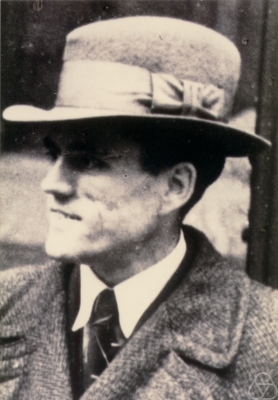
\includegraphics[width=10ex]{gentzen}\\[-1ex]
		{\tiny $\textcopyright$ Eckart Menzler-Trott, Gerhard Gentzen, \texttt{CC BY-SA 2.0 DE}}
		\end{tabular}
		\vspace{2ex}
		
		 $p\lor q,\neg q\vdash_N p$
		\end{center}
		
		
\begin{center}
			\begin{tabular}{c}
				\infer[\lor E, 1]{q}{p\lor q & [q] &\infer[EFQ]{q}{[p] & \neg q}}
			\end{tabular}
		\end{center}	
\end{frame}


\subsection{6.2 Satisfiability and Consequence}

\begin{frame}{6.2 Satisfiability and Consequence}

	\begin{itemize}
	
		\item (6.1.1) The method of analytic tableaux is based on a theorem (just like the truth-tables).
	
		\item	(6.2.2)  A set of formulas $\Gamma\subseteq\mathcal{L}$ is said to be satisfiable iff there exists a valuation $v$ such that $\llbracket\phi\rrbracket_v=1$ for all $\phi\in\Gamma$.
		
		\item (6.2.3) \emph{Examples}:
		
			\begin{enumerate}[(a)]
			
				\item $\mathcal{P}$
				
				\item $X\subseteq\mathcal{P}$
				
				\item$\emptyset$!
				
				\item \textbf{Proposition}. Let $\Gamma,\Delta\subseteq\mathcal{L}$ be sets of formulas. If $\Gamma$ is satisfiable and $\Delta\subseteq \Gamma$, then $\Delta$ is satisfiable.				
				\item[] \emph{Proof (Sketch).} If $\Gamma$ is satisfiable, then there's a valuation that makes all the $\Gamma$'s true. But if $\Delta\subseteq\Gamma$, then all the $\Delta$'s are also $\Gamma$'s. Hence also $\Delta$ is satisfiable.
			
				\item $\{p\lor\neg p\}$
			
				\item $\{p\to q, \neg q\}$ is satisfiable with $v(p)=0$ and $v(q)=0$
			
			\end{enumerate}
	
	\end{itemize}

\end{frame}

\begin{frame}{\emph{Un}satisfiability}
	
	\begin{itemize}

		\item (6.2.4) A set $\Gamma$ is \emph{un}satisfiable iff there exists no valuation $v$ such that $\llbracket\phi\rrbracket_v=1$ for all $\phi\in\Gamma$.
		
		\item (6.2.5) \emph{Examples}:
		
			\begin{enumerate}[(a)]
			
				\item $\{\phi,\neg\phi\}$ (Reason: if $\llbracket\phi\rrbracket_v=1$ and $\llbracket\neg \phi\rrbracket_v=1$, it follows that $\llbracket\phi\rrbracket_v=1$ or $\llbracket\phi\rrbracket_v=0$ \lightning)
				
				\item $\mathcal{L}$!
				
				\item \textbf{Proposition}. Let $\Gamma,\Delta\subseteq\mathcal{L}$ be sets of formulas. If $\Gamma$ is unsatisfiable and $\Gamma\subseteq \Delta$, then $\Delta$ is unsatisfiable.
				
				\item[] \emph{Proof (Sketch)}. If $\Delta$ would be satisfiable, then there'd be a valuation $v$ that makes all the $\Delta$'s true. But if $\Gamma\subseteq\Delta$, then all the $\Gamma$'s are $\Delta$'s and so $v$ would make all the $\Gamma$'s true. But that's a contradiction to $\Gamma$ being unsatisfiable.
				
				\item $\{p\lor q, \neg p, \neg q\}$ (Reason: $\llbracket\neg p\rrbracket_v=1$ means $\llbracket p\rrbracket_v=0$, $\llbracket\neg q\rrbracket_v=1$ means $\llbracket q\rrbracket_v=0$, and $\llbracket p\lor q\rrbracket_v=1$ means that either $\llbracket p\rrbracket_v=1$ or $\llbracket q\rrbracket_v=1$. \lightning)
			
			\end{enumerate}
	
	\end{itemize}

\end{frame}

\begin{frame}{The ``I Can't Get No Satisfaction''--Theorem}

	\begin{itemize}
		
		\item \textbf{Theorem}. Let $\Gamma\subseteq\mathcal{L}$ be a set of formulas and $\phi\in\mathcal{L}$ a formula. Then, the following are equivalent:
			\begin{enumerate}[1.]
			
				\item $\Gamma\vDash\phi$
				
				\item $\Gamma\cup\{\neg\phi\}$ is unsatisfiable
			
			\end{enumerate}
			
		\item \emph{Proof}:
		
			\begin{itemize}
			
				\item ($1.\Rightarrow 2.$) Suppose that $\Gamma\vDash\phi$. We prove indirectly that $\Gamma\cup\{\neg\phi\}$ is unsatisfiable. So, suppose that  $\Gamma\cup\{\neg\phi\}$  is satisfiable by $v$. Then $v$ makes all the members of $\Gamma$ and $\neg\phi$ true. Since $\Gamma\vDash\phi$, this means that $v$ makes $\phi$ true. But now we have that both $\phi$ and $\neg\phi$ are true, which is impossible. Hence $\Gamma\cup\{\neg\phi\}$ is unsatisfiable.
				
				\item ($2.\Rightarrow 1.$) Suppose that $\Gamma\cup\{\neg\phi\}$ is unsatisfiable. We prove that $\Gamma\vDash\phi$ indirectly. For suppose that $\Gamma\nvDash\phi$, i.e. there exists a valuation $v$ that makes all the $\Gamma$'s true and $\phi$ false. But if $\phi$ is false under $v$, then $\neg\phi$ is true. So $v$ makes all the $\Gamma$'s and $\neg\phi$ true, which means that $\Gamma\cup\{\neg\phi\}$ is satisfiable---in contradiction to our assumption that it's not.
			
			\end{itemize}

	\end{itemize}

\end{frame}

\subsection{6.3 Analytic Tableaux}

\begin{frame}{6.3 Analytic Tableaux}

	\begin{itemize}
		
		\item (6.3.1) Analytic tableaux are a method for determining satisfiability. 
		
		\item This allows us to determine consequence using the ICGNS-theorem. 
		
		\item In contrast to truth-tables, tableaux are purely syntactic.
		
		\item We describe it step-by-step:
		
		\begin{enumerate}[1.]
		
			\item We begin by writing down the members of $\Gamma$ as the \emph{initial list}. This list forms the root of our tableau.
			
			\item[] \emph{Examples}.
			
			\begin{itemize}

				\item $\Gamma=\{p\lor q, \neg p, \neg q\}$

				\item[] Initial List: 

					\begin{prooftree}
						{
						line numbering=false,
						line no sep= 2cm,
						for tree={s sep'=5mm},
						single branches=true,
						close with=\xmark
						}
						[p\lor q, grouped [\neg p, grouped [\neg q, grouped] ] ]
					\end{prooftree}
					
				\item $\Gamma=\{p\land q, \neg p\lor q, \neg (q\land \neg \neg r)\}$

					\item[] Initial List:

					\begin{prooftree}
					{
					line numbering=false,
					line no sep= 2cm,
					for tree={s sep'=5mm},
					single branches=true,
					close with=\xmark
					}
					[p\land q, grouped [ \neg p\lor q, grouped [\neg (q\land \neg \neg r), grouped ] ] ]
					\end{prooftree}
					

			\end{itemize}
		
		\end{enumerate}
	
	\end{itemize}

\end{frame}

\begin{frame}{Tableaux --- \emph{How To}}

	\begin{enumerate}
	\setcounter{enumi}{1}
	
	\item Next, we repeatedly apply the following rules: 
					\vspace{2ex}
				
					\begin{center}
							{\tiny		
	
					\begin{prooftree}
					{
					line numbering=false,
					line no sep= 2cm,
					for tree={s sep'=5mm},
					single branches=true,
					close with=\xmark
					}
					[\neg\neg \phi [\phi ] ]
					\end{prooftree}
					%
					\begin{prooftree}
					{
					line numbering=false,
					line no sep= 2cm,
					for tree={s sep'=5mm},
					single branches=true,
					close with=\xmark
					}
					[\phi\land\psi [\phi [\psi ] ] ]
					\end{prooftree}
					%
					\begin{prooftree}
					{
					line numbering=false,
					line no sep= 2cm,
					for tree={s sep'=5mm},
					single branches=true,
					close with=\xmark
					}
					[\neg (\phi\land\psi) [\neg \phi ] [\neg \psi ] ]
					\end{prooftree}
					%
					\begin{prooftree}
					{
					line numbering=false,
					line no sep= 2cm,
					for tree={s sep'=5mm},
					single branches=true,
					close with=\xmark
					}
					[\phi\lor\psi [\phi ] [\psi ] ]
					\end{prooftree}
					%
					\begin{prooftree}
					{
					line numbering=false,
					line no sep= 2cm,
					for tree={s sep'=5mm},
					single branches=true,
					close with=\xmark
					}
					[\neg(\phi\lor\psi) [\neg\phi [\neg\psi ] ] ]
					\end{prooftree}

					\vspace{2ex}

					\begin{prooftree}
					{
					line numbering=false,
					line no sep= 2cm,
					for tree={s sep'=5mm},
					single branches=true,
					close with=\xmark
					}
					[\neg (\phi\to\psi) [\phi [\neg \psi ] ] ]
					\end{prooftree}
					%
					\begin{prooftree}
					{
					line numbering=false,
					line no sep= 2cm,
					for tree={s sep'=5mm},
					single branches=true,
					close with=\xmark
					}
					[\phi\to\psi [\neg \phi ] [\psi ] ]
					\end{prooftree}
					%
					\begin{prooftree}
					{
					line numbering=false,
					line no sep= 2cm,
					for tree={s sep'=5mm},
					single branches=true,
					close with=\xmark
					}
					[\phi\leftrightarrow \psi [\phi [\psi] ] [\neg \phi [\neg \psi] ] ]]
					\end{prooftree}
					%
					\begin{prooftree}
					{
					line numbering=false,
					line no sep= 2cm,
					for tree={s sep'=5mm},
					single branches=true,
					close with=\xmark
					}
					[\neg(\phi\leftrightarrow \psi) [\phi [\neg \psi] ] [\neg \phi [ \psi] ] ]]
					\end{prooftree}}

				\end{center}
			We read these rules as follows:
			
				\begin{itemize}
		
			\item If there's a node with a formula to which no rule has been applied yet, then we apply the rule by extending every branch that goes through the node as shown by the rule.
			
			\end{itemize}
			
			 If all the rules that can be applied have been applied, then we say that the tableau is \emph{complete}.
	
	\end{enumerate}

\end{frame}

\begin{frame}{Examples}

\begin{center}
					\begin{prooftree}
					{
					line numbering=false,
					line no sep= 2cm,
					for tree={s sep'=5mm},
					single branches=true,
					close with=\xmark
					}
					[p\lor q, grouped [\neg p, grouped [\neg q, 					grouped [p] [q] ] ] ]
					\end{prooftree}
					\qquad
					\begin{prooftree}
					{
					line numbering=false,
					line no sep= 1cm,
					for tree={s sep'=5mm},
					single branches=true,
					close with=\xmark
					}
					[p\land q, grouped [ \neg p\lor q, grouped [\neg (q\land \neg\neg r), grouped [p [q [\neg p [\neg q] [\neg\neg\neg r [\neg r] ] ] [q [\neg q] [\neg\neg\neg r [\neg r] ] ] ] ] ] ] ]
					\end{prooftree}
				\end{center}


\end{frame}

\begin{frame}{Tableaux --- \emph{How To}}

	\begin{enumerate}
	\setcounter{enumi}{2}
	
		 \item Once we've completed our tableau, we check on every branch $B$ whether there is a $p\in\mathcal{P}$ such that $p\in B$ and $\neg p\in B$.
			
			\begin{itemize}
		
			\item if yes, then we say that $B$ is \emph{closed}, and mark it by writing an {\xmark} under it;
			
			\item if no, then we say that $B$ is \emph{open}. 
		
		\end{itemize}
	
	\end{enumerate}

\begin{center}
{\tiny\begin{prooftree}
{
line numbering=false,
line no sep= 2cm,
for tree={s sep'=5mm},
single branches=true,
close with=\xmark
}
[p\lor q, grouped [\neg p, grouped [\neg q, grouped [p, close] [q, close] ] ] ]
\end{prooftree}
\qquad\begin{prooftree}
{
line numbering=false,
line no sep= 1cm,
for tree={s sep'=5mm},
single branches=true,
close with=\xmark
}
[p\land q, grouped [ \neg p\lor q, grouped [\neg (q\land \neg\neg r), grouped [p [q [\neg p [\neg q, close] [\neg\neg\neg r [\neg r, close] ] ] [q [\neg q, close] [\neg\neg\neg r [\neg r ] ] ] ] ] ] ] ]
\end{prooftree}}
\end{center}

\end{frame}

\begin{frame}{Tableaux --- \emph{How To}}

	\begin{enumerate}
	\setcounter{enumi}{3}
	
		\item We now check our tableau whether there an open branch in the tree (i.e. a branch without an {\xmark} underneath):			
			\begin{itemize}
			
				\item If yes, the tableau is called \emph{open} and the set is satisfiable.
				
				\item If no, the tableau is called \emph{closed} and the set is unsatisfiable.
			
			\end{itemize}	
	\end{enumerate}
	
\begin{center}
{\tiny\begin{prooftree}
{
line numbering=false,
line no sep= 2cm,
for tree={s sep'=5mm},
single branches=true,
close with=\xmark
}
[p\lor q, grouped [\neg p, grouped [\neg q, grouped [p, close] [q, close] ] ] ]
\end{prooftree}
\qquad\begin{prooftree}
{
line numbering=false,
line no sep= 1cm,
for tree={s sep'=5mm},
single branches=true,
close with=\xmark
}
[p\land q, grouped [ \neg p\lor q, grouped [\neg (q\land \neg\neg r), grouped [p [q [\neg p [\neg q, close] [\neg\neg\neg r [\neg r, close] ] ] [q [\neg q, close] [\neg\neg\neg r [\neg r ] ] ] ] ] ] ] ]
\end{prooftree}}
\end{center}
	
\end{frame}

\begin{frame}{Tableaux --- The Idea}

	\begin{itemize}
	
		\item (6.3.3.) The rules allow us to test, step-by-step, what would need to be the case for the formulas in the tree to be true. A rule creates new branches if there's more than one possibility for the formula to be true:
		
		\begin{description}
			
				\item[Down Preservation.] If the formula $\phi$ at the parent node of a rule is true under a valuation $v$, then at least one formula $\psi$ on a newly generated child node is true under $v$.
				
				\begin{center}{\tiny
					\begin{prooftree}
					{
					line numbering=false,
					line no sep= 2cm,
					for tree={s sep'=5mm},
					single branches=true,
					close with=\xmark
					}
					[\neg (\phi\to\psi) [\phi [\neg \psi ] ] ]
					\end{prooftree}
					%
					\begin{prooftree}
					{
					line numbering=false,
					line no sep= 2cm,
					for tree={s sep'=5mm},
					single branches=true,
					close with=\xmark
					}
					[\phi\lor\psi [\phi ] [\psi ] ]
					\end{prooftree}}
				\end{center}
				
				\item[Up Preservation.] If a formula $\psi$ at a newly generated child node is true under $v$, then the formula $\phi$ at the parent node is true.
			
			\end{description}
	
	\end{itemize}

\end{frame}

\begin{frame}{Associated Interpretations and Closure}

	\begin{itemize}
	
		\item (6.3.3) Each branch $B$ corresponds to a valuation $v_B$ such that $\llbracket\phi\rrbracket_{v_B}=1$ whenever $\phi\in B$.
		
		\item (6.3.4) If both $p,\neg p\in B$, then there can't be such a valuation $v_B$. Hence we close the branch. 
		
		%\item In this way, we go through all the possibilities. Hence, if we only find \xmark's, we know that there is no interpretation that makes all the formulas on the branch true.
		
		\item (6.3.5) If $B$ is an open branch of a tableau, then we define $v_B:\mathcal{P}\to\{0,1\}$ by setting:\[v_B(p):=\begin{cases} 1 &\text{if }p\in B\\0&\text{if }p\notin B\end{cases}\]	
		
		\item \textbf{Theorem} (to be proven later). Let $B$ be an open branch of a complete tableau and $v_B$ its associated valuation. Then for all $\phi\in B$, we have that $\llbracket\phi\rrbracket_{v_B}=1$.
	
	\end{itemize}

\end{frame}

\begin{frame}{Example}

		\begin{center}
{\small\begin{prooftree}
{
line numbering=false,
line no sep= 2cm,
for tree={s sep'=5mm},
single branches=true,
close with=\xmark
}
[p\land q, grouped [ \neg p\lor q, grouped [\neg (q\land \neg\neg r), grouped [p [q [\neg p [\neg q, close] [\neg\neg\neg r [\neg r, close] ] ] [q [\neg q, close] [\neg\neg\neg r [\neg r ] ] ] ] ] ] ] ]
\end{prooftree}}
\end{center}

	There's only one open branch $B$ (the right-most one), $v_B$ is given by $v_B(p)=1, v_B(q)=1, v_B(r)=0$.

\end{frame}

\begin{frame}{From (Un)Satisfiability Checking to Provability}

	\begin{itemize}
	
		\item (6.3.7) Note that $\Gamma$ is on every branch (it's the root). 
		
		\item Hence if there's an open branch $B$, then $\Gamma\subseteq B$. 
		
		\item This means that $v_B$ makes all the members of $\Gamma$ true.
		
		\item Using the ICGNS-theorem, we can use tableaux to determine whether $\Gamma\vDash\phi$ by doing the tableau for $\Gamma\cup\{\neg\phi\}$.
		
		\item (6.3.8) $\Gamma\vdash_T \phi$ iff the complete tableau for $\Gamma\cup\{\neg\phi\}$ is closed.
		
		\item It follows that $\Gamma\nvdash_T \phi$ iff the complete tableau for $\Gamma\cup\{\neg\phi\}$ is open.
		
		\item The complete tableau is our proof. If it's open, we get a countermodel for free.
	
	\end{itemize}

\end{frame}

\begin{frame}{Example 1 --- De Morgan 1}

{\begin{center}
\begin{prooftree}
{
proof statement format={centered},
to prove={\neg p\lor \neg q\vdash \neg (p\land q)},
line numbering=false,
for tree={s sep'=10mm},
single branches=true,
close with=\xmark
}
[\neg p\lor \neg q, grouped [\neg \neg (p\land q), grouped [p\land q [\neg p [p [q, close] ]] [\neg q [p [q, close] ]]] ] ]
\end{prooftree}
\begin{prooftree}
{
proof statement format={centered},
to prove={\neg (p\land q)\vdash \neg p\lor \neg q},
line numbering=false,
for tree={s sep'=10mm},
single branches=true,
close with=\xmark
}
[\neg (p\land q), grouped [\neg(\neg p\lor \neg q), grouped [\neg\neg p [\neg\neg q [\neg p [p [q, close ] ] ] [\neg q [p [q, close]] ]] ]]]
\end{prooftree}
\end{center}}

\end{frame}

\begin{frame}{Example 2 -- De Morgan 2}

\begin{center}
\begin{prooftree}
{
proof statement format={centered},
to prove={\neg p\land \neg q\vdash \neg (p\lor q)},
line numbering=false,
for tree={s sep'=10mm},
single branches=true,
close with=\xmark
}
[\neg p\land \neg q, grouped [\neg \neg (p\lor q), grouped [p\lor q [ p [\neg p [\neg q, close]]] [q [\neg p [\neg q, close] ]]] ] ]
\end{prooftree}
\begin{prooftree}
{
proof statement format={centered},
to prove={\neg (p\lor q)\vdash \neg p\land \neg q},
line numbering=false,
for tree={s sep'=10mm},
single branches=true,
close with=\xmark
}
[\neg (p\lor q), grouped [\neg(\neg p\land \neg q), grouped [\neg p [\neg q [\neg \neg p [p, close]] [\neg \neg q [q, close]] ]] ]]
\end{prooftree}
\end{center}

\end{frame}

\begin{frame}{Example 3 --- Law of Excluded Middle}

\begin{center}
\begin{prooftree}
{
proof statement format={centered},
to prove={\vdash p\lor \neg p},
line numbering=false,
for tree={s sep'=10mm},
single branches=true,
close with=\xmark
}
[\neg(p\lor \neg p) [\neg p [\neg\neg p [p, close]] ] ]
\end{prooftree}
\end{center}

\end{frame}

\begin{frame}{Example 4 --- Definition of Conditional}


\begin{center}
\begin{prooftree}
{
proof statement format={centered},
to prove={\vdash (\neg p\lor q)\leftrightarrow (p\to q)},
line numbering=false,
for tree={s sep'=10mm},
single branches=true,
close with=\xmark
}
[\neg((\neg p\lor q)\leftrightarrow (p\to q)) [(\neg p\lor q) [\neg  (p\to q) [p [\neg q [\neg p, close] [q, close]] ]  ]] [\neg(\neg p\lor q) [(p\to q) [\neg\neg p [\neg q [\neg p [p, close ] ] [q [p, close ] ] ]] ] ] ]
\end{prooftree}
\end{center}

\end{frame}

\begin{frame}{Example 5 --- Transitivity}

\begin{center}
\begin{prooftree}
{
proof statement format={centered},
to prove={(p\to q), (q\to r)\vdash (p\to r)},
line numbering=false,
for tree={s sep'=10mm},
single branches=true,
close with=\xmark
}
[p\to q, grouped [q\to r, grouped [\neg (p\to r), grouped [p [\neg r [\neg p [\neg q, close] [r, close] ] [q [\neg q, close] [r, close]] ] ]] ] ]
\end{prooftree}
\end{center}

\end{frame}

\begin{frame}{Example 6 --- Distributivity}

{\scriptsize\begin{center}
\begin{prooftree}
{
proof statement format={centered},
to prove={(p\lor q)\land r\vdash (p\land r)\lor (q\land r)},
line numbering=false,
for tree={s sep'=10mm},
single branches=true,
close with=\xmark
}
[(p\lor q)\land r, grouped [\neg((p\land r)\lor (q\land r)), grouped [p\lor q [r [\neg (p\land r) [\neg (q\land r) [p [\neg p [\neg q,close] [\neg r, close]] [\neg r [\neg q,close] [\neg r, close]]] [q [\neg p [\neg q,close] [\neg r, close]] [\neg r [\neg q,close] [\neg r, close]]]]]]]]]
\end{prooftree}
\end{center}}

\end{frame}

\begin{frame}{Example 7 --- Fallacy Affirming the Consequent}

\begin{center}
\begin{prooftree}
{
proof statement format={centered},
to prove={p\to q, q\nvdash p},
line numbering=false,
for tree={s sep'=10mm},
single branches=true,
close with=\xmark
}
[p\to q, grouped [q, grouped [\neg p, grouped [\neg p] [q]]]]
\end{prooftree}
\end{center}

\begin{itemize}[<+->]

\item Countermodel: $v(q)=1, v(p)=0$.

\end{itemize}

\end{frame}

\begin{frame}{Example 8 --- Fallacy of Affirming the Disjunct}

\begin{center}
\begin{prooftree}
{
proof statement format={centered},
to prove={p\lor q, p\nvdash \neg q},
line numbering=false,
for tree={s sep'=10mm},
single branches=true,
close with=\xmark
}
[p\lor q, grouped [p, grouped [\neg\neg q, grouped [q [p] [q]] ]]]
\end{prooftree}
\end{center}

\begin{itemize}[<+->]
\item Countermodel: $v(p)=1, v(q)=1$.

\end{itemize}

\end{frame}

\begin{frame}{Example 9 --- Messed-Up Distributivity}


{\tiny\begin{center}
\begin{prooftree}
{
proof statement format={centered},
to prove={(p\lor r)\land (q\lor r)\nvdash (p\lor q)\land r},
line numbering=false,
for tree={s sep'=10mm},
single branches=true,
close with=\xmark
}
[(p\lor r)\land (q\lor r), grouped [\neg((p\lor q)\land r), grouped  [p\lor r [q\lor r [\neg(p\lor q) [\neg p [\neg q [p [q,close] [r, close]] [r[q,close] [r]]]]] [\neg r [p [q] [r, close ]] [r [q,close] [r, close]]]] ] ]] ]
\end{prooftree}
\end{center}}

\begin{itemize}[<+->]
\item Countermodel: $v(p)=0, v(q)=0, v(r)=1$.

\end{itemize}

\end{frame}
\begin{frame}{Core Ideas (Lecture Version)}
 
\begin{itemize}

	\item There are several different \emph{kinds} of proof systems: Hilbert calculi, sequent calculi, natural deduction, and analytic tableaux. In this course, we use analytic tableaux. 
	
	\item A set of formulas is satisfiable iff there is a valuation that makes all of its members true.
	
	\item An inference is valid iff the set of the premises and the negation of the conclusion is unsatisfiable.
	
	\item The method of analytic tableaux is an algorithm for checking whether a set of formulas is satisfiable: if the tableau for a set is open, then the set is satisfiable.
	
	\item We define a proof system using analytic tableaux by defining derivability as the tableau for the set of premises plus negation of conclusion being closed.
	
	\item We can read-off a countermodel from an open branch of an open tableau.

\end{itemize}


\end{frame}

\section{Exam}

\begin{frame}{Exam}

\begin{center}
		
\includegraphics[width=40ex]{xkcd-students}\\
		{\tiny \textcopyright~\url{https://xkcd.com/557/}, CC BY-NC 2.5}
		\end{center}
	

	\begin{itemize}
	
		\item Digital
	
		\item Multiple-choice/fill-in-the-gaps/etc.
		
		\item Questions formulated both in English and Dutch.
		
		\item Tests understanding of core concepts (see next slide).
		
		\item Length: \textbf{2 hours} (+extra time)!
		
		\item Q\&A next Tuesday.
	
	\end{itemize}

\end{frame}

\begin{frame}{Core concepts}

	\begin{description}
	
		\item[\S1. Introduction] \
		
			\begin{itemize}
			
				\item Validity as truth-preservation across all situations
				
				\item Logical truth as truth in all situations
				
				\item Bivalence 
								
				\item Soundness and Completeness
				
				\item Decidability
			
			\end{itemize}
	
		\item[\S2. Mathematics] \
		
			\begin{itemize}
			
				\item Variables vs. Constants
				
				\item Definitions of objects (uniqueness + existence)
				
				\item Definitions of properties and relations (non-circular)
				
				\item Concept of informal rigor
			
			\end{itemize}
	
	\end{description}

\end{frame}

\begin{frame}{Core concepts}

	\begin{description}
	
		\item[\S3. Set Theory] \
		
			\begin{itemize}
			
				\item Extensional definitions and class abstracts.
				
				\item Subset relation and the power set
				
				\item Axiom of extensionality
				
				\item Set-theoretical operations: $\cup,\cap,\setminus$
				
				\item Ordered tuples and Cartesian products
				
				\item Properties and relations
				
				\item Functions
				
				\item Inductive definitions, function recursion, proof by induction
			
			\end{itemize}
	
		\item[\S4. Syntax] \
		
			\begin{itemize}
													
				\item Formalization
				
				\item Parsing trees
				
				\item Syntactic recursion
				
				\item Unique readability theorem
				
				\item Criteria for formula-hood
			
				\item Conventional notation
			
			\end{itemize}
	
	\end{description}

\end{frame}

\begin{frame}{Core concepts}

	\begin{description}
	
		\item[\S5. Semantics] \
		
			\begin{itemize}
			
				\item Valuations as situations
				
				\item Recursive definition of truth
				
				\item Validity of inferences as truth-preservation across valuations
				
				\item Logical truth as consequence of $\emptyset$
				
				\item The reduction of validity to logical truth
				
				\item The method of truth-tables
			
				\item Decidability of propositional logic
			
			\end{itemize}
	
		\item[\S6. Tableaux] \
		
			\begin{itemize}
									
				\item Different proof systems
				
				\item Reduction of validity to satisfiability
				
				\item Complete, open, and closed tableaux
				
				\item Associated valuations
				
				\item Definition of $\vdash_T$
			
			\end{itemize}
	
	\end{description}

\end{frame}

\begin{frame}

	\begin{center}
	{\huge\bf Thanks!}
	\end{center}

\end{frame}

